\documentclass{beamer}
\usepackage{siunitx}
\let\vec\mathbf
\mode<presentation>
\usepackage{amsmath}
\usepackage{amssymb}
%\usepackage{advdate}
\usepackage{adjustbox}
%\usepackage{subcaption}
\usepackage{enumitem}
\usepackage{multicol}
\usepackage{mathtools}
\usepackage{listings}
\usepackage{url}
\usetheme{Boadilla}
\usecolortheme{lily}
\setbeamertemplate{footline}
{
  \leavevmode%
  \hbox{%
  \begin{beamercolorbox}[wd=\paperwidth,ht=2.25ex,dp=1ex,right]{author in head/foot}%
    \insertframenumber{} / \inserttotalframenumber\hspace*{2ex} 
  \end{beamercolorbox}}%
  \vskip0pt%
}
\setbeamertemplate{navigation symbols}{}
\providecommand{\nCr}[2]{\,^{#1}C_{#2}} % nCr
\providecommand{\nPr}[2]{\,^{#1}P_{#2}} % nPr
\providecommand{\mbf}{\mathbf}
\providecommand{\pr}[1]{\ensuremath{\Pr\left(#1\right)}}
\providecommand{\qfunc}[1]{\ensuremath{Q\left(#1\right)}}
\providecommand{\sbrak}[1]{\ensuremath{{}\left[#1\right]}}
\providecommand{\lsbrak}[1]{\ensuremath{{}\left[#1\right.}}
\providecommand{\rsbrak}[1]{\ensuremath{{}\left.#1\right]}}
\providecommand{\brak}[1]{\ensuremath{\left(#1\right)}}
\providecommand{\lbrak}[1]{\ensuremath{\left(#1\right.}}
\providecommand{\rbrak}[1]{\ensuremath{\left.#1\right)}}
\providecommand{\cbrak}[1]{\ensuremath{\left\{#1\right\}}}
\providecommand{\lcbrak}[1]{\ensuremath{\left\{#1\right.}}
\providecommand{\rcbrak}[1]{\ensuremath{\left.#1\right\}}}
\theoremstyle{remark}
\newtheorem{rem}{Remark}
\newcommand{\sgn}{\mathop{\mathrm{sgn}}}

\providecommand{\res}[1]{\Res\displaylimits_{#1}} 
\providecommand{\norm}[1]{\left\lVert#1\right\rVert}
\providecommand{\mtx}[1]{\mathbf{#1}}
\providecommand{\abs}[1]{\left\vert#1\right\vert}
\providecommand{\fourier}{\overset{\mathcal{F}}{ \rightleftharpoons}}
%\providecommand{\hilbert}{\overset{\mathcal{H}}{ \rightleftharpoons}}
\providecommand{\system}{\overset{\mathcal{H}}{ \longleftrightarrow}}
	%\newcommand{\solution}[2]{\textbf{Solution:}{#1}}
%\newcommand{\solution}{\noindent \textbf{Solution: }}align
\providecommand{\dec}[2]{\ensuremath{\overset{#1}{\underset{#2}{\gtrless}}}}
\newcommand{\myvec}[1]{\ensuremath{\begin{pmatrix}#1\end{pmatrix}}}

\title{Matrices in Geometry - 5.2.40}
\author{EE25BTECH11037  Divyansh}
\date{Sept, 2025}

\begin{document}

\maketitle


\section{Problem}
\begin{frame}
\frametitle{Problem Statement}
Solve
\begin{align*}
    \frac{4}{x}+3y=14 \\
    \frac{3}{x} -4y =23
\end{align*}
\end{frame}

\section{Solution}
\begin{frame}{Solution}
   
We have the following two equations as:
\begin{align}
    \myvec{4 & 3 \\ 3 & -4}\myvec{\frac{1}{x} \\ y}=\myvec{14 \\ 23}
\end{align}
Writing the augmented matrix for these equations,
\begin{align}
    \myvec{4 & 3 & \vrule & 14 \\ 3 & -4 & \vrule & 23} \overset{R_1 \rightarrow R_1 /4}{\longleftrightarrow} \myvec{1 & 3/4 & \vrule & 7/2 \\ 3 & -4 & \vrule & 23}\overset{R_2 \rightarrow R_2-3R_1}{\longleftrightarrow} \\\myvec{1 & 3/4 & \vrule & 7/2 \\ 0 & -25/4 & \vrule & 25/2} \overset{R_2 \rightarrow \frac{-4}{25}R_2}{\longleftrightarrow} \myvec{1 & 3/4 & \vrule & 7/2 \\ 0 & 1 & \vrule & -2}\overset{R_1 \rightarrow R_1-\frac{3}{4} R_2}{\longleftrightarrow}\\ \myvec{1 & 0 & \vrule & 5 \\ 0 & 1 & \vrule & -2}
\end{align}

\end{frame}

\begin{frame}{Solution}
This implies that
\begin{align}
    \myvec{\frac{1}{x} \\ y} = \myvec{5 \\ -2}\implies x=\dfrac{1}{5} \ , \ y=-2
\end{align}
\begin{figure}[H]
    \centering
    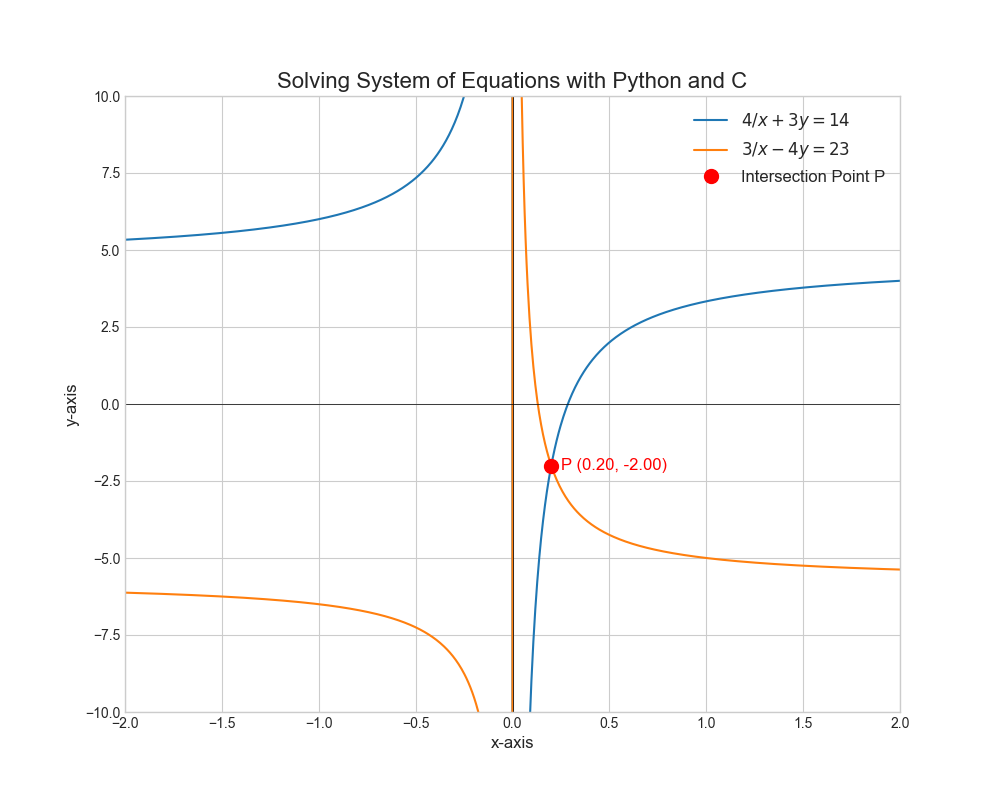
\includegraphics[width=0.5\columnwidth]{figs/1.png}
    \caption{Graph for 5.2.40}
    \label{fig:placeholder}
\end{figure}  
\end{frame}



\end{document}